\documentclass{article}
\usepackage[utf8]{inputenc}
\usepackage{amsmath}
\usepackage{amssymb}
\usepackage{physics}
\usepackage{gensymb}
\usepackage{simpler-wick}
\usepackage{tikz}
\usepackage[compat=1.1.0]{tikz-feynman}
\usepackage{esvect}
\usepackage[title]{appendix} % or other options
\usepackage{graphicx} % Required for inserting images

% Custom commands for partial derivatives
\newcommand{\pd}{\partial}  % Short for \partial
\newcommand{\pdm}{\partial_\mu}  % \partial_\mu
\newcommand{\pdn}{\partial_\nu}  % \partial_\nu
\newcommand{\pdup}{\partial^\mu}  % \partial^\mu
\newcommand{\pdupnu}{\partial^\nu}  % \partial^\nu
\newcommand{\Lag}{\mathcal{L}}  % Lagrangian shorthand
\newcommand{\onehalf}{\frac{1}{2}}
\newcommand{\pdotx}{\vec{p}.\vec{x}}
\newcommand{\qdotx}{\vec{q}.\vec{x}}
\newcommand{\sdotx}{\vec{s}.\vec{x}}
\newcommand{\qdoty}{\vec{q}.\vec{y}}
\newcommand{\asp}{a_{\vec{p}}}
\newcommand{\ass}{a_{\vec{s}}}
\newcommand{\asq}{a_{\vec{q}}}
\newcommand{\adp}{a_{\vec{p}}^\dagger}
\newcommand{\adq}{a_{\vec{q}}^\dagger}
\newcommand{\ads}{a_{\vec{s}}^\dagger}

\newcommand{\phionep}{\phi_1^+}
\newcommand{\phionem}{\phi_1^-}
\newcommand{\phitwop}{\phi_2^+}
\newcommand{\phitwom}{\phi_2^-}
\newcommand{\phithreep}{\phi_3^+}
\newcommand{\phithreem}{\phi_3^-}

\newcommand{\vecx}{\vec{x}}
\newcommand{\vecy}{\vec{y}}
\newcommand{\vecp}{\vec{p}}
\newcommand{\vecq}{\vec{q}}
\newcommand{\vecs}{\vec{s}}

% Alternative shorter versions
\newcommand{\dmu}{\partial_\mu}
\newcommand{\dnu}{\partial_\nu}
\newcommand{\dmuup}{\partial^\mu}
\newcommand{\dnuup}{\partial^\nu}
\newcommand{\lagden}{\mathcal{L}}
% Even shorter versions (if you prefer)
\newcommand{\dm}{\partial_\mu}
\newcommand{\dn}{\partial_\nu}
\newcommand{\dmuu}{\partial^\mu}
\newcommand{\dnuu}{\partial^\nu}
\newcommand{\lagrangian}{\mathcal{L}}

\title{My Solutions to Problem Sheet 2 QFT by David Tong}
\author{Baset}
\date{October 2025}

\begin{document}

\maketitle
\section*{1.}
According to the definitions made:
\begin{equation}
    \begin{split}
    [a_n,a_m] &= [\sqrt{\frac{\omega_n}{2}}q_n+\frac{i}{\sqrt{2\omega_n}}p_n,
    \sqrt{\frac{\omega_m}{2}}q_m+\frac{i}{\sqrt{2\omega_m}}p_m]\\
    &= \onehalf \{ i[q_n,p_m] + i[p_n,q_m] \} = 0
    \end{split}
\end{equation}

\begin{equation}
    \begin{split}
    [a_n,a_m] &= [\sqrt{\frac{\omega_n}{2}}q_n+\frac{i}{\sqrt{2\omega_n}}p_n,
    \sqrt{\frac{\omega_m}{2}}q_m+\frac{i}{\sqrt{2\omega_m}}p_m]\\
    &= \onehalf \{ i[q_n,p_m] + i[p_n,q_m] \} = 0
    \end{split}
\end{equation}

\begin{equation}
    \begin{split}
    [a_n^\dagger,a_m^\dagger] &= [\sqrt{\frac{\omega_n}{2}}q_n-\frac{i}{\sqrt{2\omega_n}}p_n,
    \sqrt{\frac{\omega_m}{2}}q_m-\frac{i}{\sqrt{2\omega_m}}p_m]\\
    &= \onehalf \{ -i[q_n,p_m] - i[p_n,q_m] \} = 0
\end{split}
\end{equation}
\begin{equation}\label{commuteofa}
    \begin{split}
    [a_n,a_m^\dagger] &= [\sqrt{\frac{\omega_n}{2}}q_n+\frac{i}{\sqrt{2\omega_n}}p_n,
    \sqrt{\frac{\omega_m}{2}}q_m-\frac{i}{\sqrt{2\omega_m}}p_m]\\
    &= \onehalf \{ -i[q_n,p_m] + i[p_n,q_m] \} =\delta_{nm}
\end{split}
\end{equation}
Using ~\ref{commuteofa}:
\begin{equation}
    \begin{split}
    H &= \sum_n \onehalf \omega_n( a_n a_n^\dagger + a_n^\dagger a_n ) = \sum_n \omega_n(a_n^\dagger a_n + \onehalf) \\
    &=  \sum_n \omega_n ((\sqrt{\frac{\omega_n}{2}}q_n-\frac{i}{\sqrt{2\omega_n}}p_n)(\sqrt{\frac{\omega_n}{2}}q_n+\frac{i}{\sqrt{2\omega_n}}p_n) + \onehalf) \\
    &= \sum_n \omega_n(\onehalf\omega_n q_n^2 + \frac{1}{2\omega_n}p_n^2 + \frac{i}{2}[q_n,p_n] + \onehalf) \\
    &= \sum_n \onehalf(p_n^2 + \omega_n^2q_n^2)
\end{split}
\end{equation}
If we use the first line of the above calculation as $H$:
\begin{equation}
    \begin{split}
        H\ket{0} = \sum_n \omega_n(a_n^\dagger a_n + \onehalf)\ket{0} = \infty\ket{0}    
    \end{split}
\end{equation}
In the above $H$ terms, the only term that produces a non-zero energy when acting on vacuum $\ket{0}$ is the constant $\onehalf$ term, by removing it:
\begin{equation}
    \begin{split}
        H\ket{0} = \sum_n\omega_na_n^\dagger a_n\ket{0} = 0\ket{0}
    \end{split}
\end{equation}

\begin{equation}
\begin{split}
    [H, a_n^\dagger]&=[\sum_{m=1}^\infty \omega_ma_m^\dagger a_m, a_n^\dagger] = \sum_{m=1}^\infty \omega_m [a_m^\dagger a_m, a_n^\dagger] \\
    & = \sum_{m=1}^\infty \omega_m a_m^\dagger [a_m,a_n^\dagger] = \omega_na_n^\dagger
    \end{split}
\end{equation}
Therefore:
\begin{equation}
    \begin{split}
        g_l \equiv [H, (a_n^\dagger)^l] &= [H,a_n^\dagger](a_n^\dagger)^{l-1} + a_n^\dagger[H,(a_n^\dagger)^{l-1}] = \omega_n(a_n^\dagger)^l + a_n^\dagger[H,(a_n^\dagger)^{l-1}]\\
        &= \omega_n(a_n^\dagger)^l + a_n^\dagger g_{l-1} = \omega_n(a_n^\dagger)^l + a_n^\dagger(\omega_n(a_n^\dagger)^{l-1}
        a_n^\dagger g_{l-2} ) \\
        &=  2\omega_n(a_n^\dagger)^l + (a_n^\dagger)^2 g_{l-2} = \dots \\
        &= l\omega_n(a_n^\dagger)^l + (a_n^\dagger)^l g_0 =  l\omega_n(a_n^\dagger)^l
    \end{split}
\end{equation}

\begin{equation}
    \begin{split}
        H\ket{l_1,l_2,...,l_N} &= H(a_1^\dagger)^{l_1}(a_2^\dagger)^{l_2}...(a_N^\dagger)^{l_N}\ket{0} \\
        & = ((a_1^\dagger)^{l_1}H + l_1\omega_1(a_1^\dagger)^{l_1})(a_2^\dagger)^{l_2}...(a_N^\dagger)^{l_N}\ket{0} \\
        & = (a_1^\dagger)^{l_1}((l_2\omega_2)(a_2^\dagger)^{l_2} + (a_2^\dagger)^{l_2}H + l_1\omega_1 (a_2^\dagger)^{l_2})
        \dots (a_N^\dagger)^{l_N}\ket{0}\\
        & = (a_1^\dagger)^{l_1} (a_2^\dagger)^{l_2} ( (l_1\omega_1 + l_2\omega_2) + H) \dots (a_N^\dagger)^{l_N}\ket{0} = \dots\\
        & = (a_1^\dagger)^{l_1} (a_2^\dagger)^{l_2}\dots (a_N^\dagger)^{l_N} (\sum l_i\omega_i + H )\ket{0} \\
        &= \sum l_i\omega_i \ket{l_1,l_2,...,l_N}
    \end{split}
\end{equation}

\section*{2.}
\begin{equation}
    \begin{split}
        [\phi(\vec{x}), \phi(\vec{y})] &= \int\int \frac{d^3p\, d^3q}{(2\pi)^6}\frac{1}{2\sqrt{E_{\vec{p}}\, E_{\vec{q}}}}[
            \asp \, e^{i\pdotx} + \asp^\dagger \, e^{-\pdotx}, \asq \, e^{i\qdoty} + \asq^\dagger \, e^{-i\qdoty}] \\
        &= \int\int d\mathcal{P}\left(  e^{i (\pdotx - \qdoty)}[\asp, \asq^\dagger] + e^{i(\qdoty - \pdotx)}[\asp^\dagger,\asq]\right)\\
        &= \int\int \frac{d^3p \, d^3q}{(2\pi)^3}\frac{1}{2\sqrt{E_{\vec{p}}\, E_{\vec{q}}}}  e^{i (\pdotx - \qdoty)} \delta(\vec{p}-\vec{q}) - \int\int 
        \frac{d^3p \, d^3q}{(2\pi)^3} \frac{1}{2\sqrt{E_{\vec{p}}\, E_{\vec{q}}}} e^{i(\qdoty - \pdotx)} \delta(\vec{q}-\vec{p})\\
        &= 0.
    \end{split}
\end{equation}


\begin{equation}
    \begin{split}
        [\pi(\vec{x}), \pi(\vec{y})] &= \int\int - \frac{d^3p \, d^3q}{(2\pi)^3}\frac{\sqrt{E_{\vec{p}}E_{\vec{q}}}}{2}[
            \asp \, e^{i\pdotx} - \asp^\dagger \, e^{-\pdotx}, \asq \, e^{i\qdoty} - \asq^\dagger \, e^{-i\qdoty}] \\
        &= \int\int d\mathcal{P}\, (-1)\, \left( e^{i (\pdotx - \qdoty)}[\asp, \asq^\dagger] + e^{i(\qdoty - \pdotx)}[\asp^\dagger,\asq]  \right)\\
        &= \int\int \frac{d^3p \, d^3q}{(2\pi)^3}\frac{\sqrt{E_{\vec{p}}\, E_{\vec{q}}}}{2\sqrt{E_{\vec{p}}\, E_{\vec{q}}}}  e^{i (\pdotx - \qdoty)} \delta(\vec{p}-\vec{q}) - \int\int 
        \frac{d^3p \, d^3q}{(2\pi)^3} \frac{\sqrt{E_{\vec{p}}\, E_{\vec{q}}}}{2} e^{i(\qdoty - \pdotx)} \delta(\vec{q}-\vec{p})\\
        &=0.
    \end{split}
\end{equation}

\begin{equation}
    \begin{split}
        [\phi(\vec{x}), \pi(\vec{y})] &= \int\int (-i) \frac{d^3p \, d^3q}{(2\pi)^3}\onehalf\sqrt{\frac{E_{\vec{q}}}{E_{\vec{p}}}}
    \end{split}
\end{equation}



%%%%%%%%%%%%%%%%%%%%%%%%%%%%%%%%%%%%%%%%%%%%%%%%
%%%%%%%%%%%%%%%%%%%%%%%%%%%%%%%%%%%%%%%%%%%%%%%%%
\section*{3.}

For the real scalar field,
\begin{equation}
    \mathcal L
    =
    \frac12 \partial_\mu\phi\,\partial^\mu\phi
    -
    \frac12 m^2\phi^2,
\end{equation}
the conjugate momentum is
\begin{equation}
    \pi=\dot\phi .
\end{equation}
The canonical energy-momentum tensor is
\begin{equation}
    T^{\mu\nu}
    =
    \partial^\mu\phi\,\partial^\nu\phi
    -
    \eta^{\mu\nu}\mathcal L .
\end{equation}
Thus
\begin{equation}
    P^\mu
    =
    \int d^3x\,T^{0\mu}.
\end{equation}
In particular,
\begin{equation}
    P^0=H
    =
    \frac12\int d^3x\,
    \left[
        \pi^2+(\nabla\phi)^2+m^2\phi^2
    \right],
\end{equation}
and
\begin{equation}
    P^i
    =
    \int d^3x\,T^{0i}
    =
    -\int d^3x\,\pi\,\partial_i\phi .
\end{equation}

At equal time we use
\begin{equation}
    \phi(\vec x)
    =
    \int\frac{d^3p}{(2\pi)^3}
    \frac{1}{\sqrt{2E_{\vec p}}}
    \left(
        a_{\vec p}e^{i\vec p\cdot\vec x}
        +
        a_{\vec p}^{\dagger}e^{-i\vec p\cdot\vec x}
    \right),
\end{equation}
and
\begin{equation}
    \pi(\vec x)
    =
    \int\frac{d^3p}{(2\pi)^3}
    (-i)\sqrt{\frac{E_{\vec p}}{2}}
    \left(
        a_{\vec p}e^{i\vec p\cdot\vec x}
        -
        a_{\vec p}^{\dagger}e^{-i\vec p\cdot\vec x}
    \right),
\end{equation}
with
\begin{equation}
    [a_{\vec p},a_{\vec q}^{\dagger}]
    =
    (2\pi)^3\delta^{(3)}(\vec p-\vec q).
\end{equation}
After substitution into \(P^\mu\), using
\begin{equation}
    E_{\vec p}^2=\vec p^{\,2}+m^2,
\end{equation}
the \(aa\) and \(a^\dagger a^\dagger\) terms cancel. After normal ordering, one obtains
\begin{equation}
    \boxed{
    P^\mu
    =
    \int\frac{d^3p}{(2\pi)^3}
    p^\mu
    a_{\vec p}^{\dagger}a_{\vec p}
    },
    \qquad
    p^0=E_{\vec p}.
\end{equation}

Now compute the commutators with the ladder operators:
\begin{equation}
    [P^\mu,a_{\vec q}]
    =
    -q^\mu a_{\vec q},
    \qquad
    [P^\mu,a_{\vec q}^{\dagger}]
    =
    q^\mu a_{\vec q}^{\dagger}.
\end{equation}
In the Heisenberg picture,
\begin{equation}
    \phi(x)
    =
    \int\frac{d^3p}{(2\pi)^3}
    \frac{1}{\sqrt{2E_{\vec p}}}
    \left(
        a_{\vec p}e^{-ip\cdot x}
        +
        a_{\vec p}^{\dagger}e^{ip\cdot x}
    \right).
\end{equation}
Therefore
\begin{equation}
\begin{split}
    [P^\mu,\phi(x)]
    &=
    \int\frac{d^3p}{(2\pi)^3}
    \frac{1}{\sqrt{2E_{\vec p}}}
    \left(
        -p^\mu a_{\vec p}e^{-ip\cdot x}
        +
        p^\mu a_{\vec p}^{\dagger}e^{ip\cdot x}
    \right).
\end{split}
\end{equation}
But
\begin{equation}
    \partial^\mu e^{-ip\cdot x}
    =
    -ip^\mu e^{-ip\cdot x},
    \qquad
    \partial^\mu e^{ip\cdot x}
    =
    ip^\mu e^{ip\cdot x}.
\end{equation}
Hence
\begin{equation}
    \boxed{
    [P^\mu,\phi(x)]
    =
    -i\partial^\mu\phi(x)
    }.
\end{equation}


\section*{4.}

In the Heisenberg picture,
\begin{equation}
    \dot O=i[H,O].
\end{equation}
For the free real scalar field,
\begin{equation}
    H
    =
    \frac12\int d^3y\,
    \left[
        \pi^2(\vec y,t)
        +
        (\nabla\phi(\vec y,t))^2
        +
        m^2\phi^2(\vec y,t)
    \right].
\end{equation}
The equal-time commutation relations are
\begin{equation}
    [\phi(\vec x,t),\phi(\vec y,t)]
    =
    [\pi(\vec x,t),\pi(\vec y,t)]
    =
    0,
\end{equation}
and
\begin{equation}
    [\phi(\vec x,t),\pi(\vec y,t)]
    =
    i\delta^{(3)}(\vec x-\vec y).
\end{equation}

First,
\begin{equation}
\begin{split}
    \dot\phi(\vec x,t)
    &=
    i[H,\phi(\vec x,t)]
    \\
    &=
    \frac{i}{2}
    \int d^3y\,
    [\pi^2(\vec y,t),\phi(\vec x,t)].
\end{split}
\end{equation}
Using
\begin{equation}
    [AB,C]=A[B,C]+[A,C]B,
\end{equation}
we get
\begin{equation}
\begin{split}
    [\pi^2(\vec y,t),\phi(\vec x,t)]
    &=
    \pi(\vec y,t)[\pi(\vec y,t),\phi(\vec x,t)]
    \\
    &\quad+
    [\pi(\vec y,t),\phi(\vec x,t)]\pi(\vec y,t)
    \\
    &=
    -2i\delta^{(3)}(\vec y-\vec x)\pi(\vec y,t).
\end{split}
\end{equation}
Therefore
\begin{equation}
    \boxed{
    \dot\phi(\vec x,t)=\pi(\vec x,t)
    }.
\end{equation}

Similarly,
\begin{equation}
\begin{split}
    \dot\pi(\vec x,t)
    &=
    i[H,\pi(\vec x,t)]
    \\
    &=
    \frac{i}{2}
    \int d^3y\,
    \left[
        [(\nabla\phi(\vec y,t))^2,\pi(\vec x,t)]
        +
        m^2[\phi^2(\vec y,t),\pi(\vec x,t)]
    \right].
\end{split}
\end{equation}
Now
\begin{equation}
    [\partial_i\phi(\vec y,t),\pi(\vec x,t)]
    =
    i\partial_i^y\delta^{(3)}(\vec y-\vec x),
\end{equation}
so
\begin{equation}
\begin{split}
    \frac{i}{2}
    \int d^3y\,
    [(\nabla\phi(\vec y,t))^2,\pi(\vec x,t)]
    &=
    -\int d^3y\,
    \partial_i^y\delta^{(3)}(\vec y-\vec x)
    \partial_i\phi(\vec y,t)
    \\
    &=
    \nabla^2\phi(\vec x,t).
\end{split}
\end{equation}
Also,
\begin{equation}
    [\phi^2(\vec y,t),\pi(\vec x,t)]
    =
    2i\delta^{(3)}(\vec y-\vec x)\phi(\vec y,t),
\end{equation}
and therefore
\begin{equation}
    \frac{i}{2}
    \int d^3y\,
    m^2[\phi^2(\vec y,t),\pi(\vec x,t)]
    =
    -m^2\phi(\vec x,t).
\end{equation}
Thus
\begin{equation}
    \boxed{
    \dot\pi(\vec x,t)
    =
    \nabla^2\phi(\vec x,t)-m^2\phi(\vec x,t)
    }.
\end{equation}

Since
\begin{equation}
    \dot\phi=\pi,
\end{equation}
we have
\begin{equation}
    \ddot\phi=\dot\pi.
\end{equation}
Therefore
\begin{equation}
    \ddot\phi
    =
    \nabla^2\phi-m^2\phi,
\end{equation}
or
\begin{equation}
    \boxed{
    (\partial_\mu\partial^\mu+m^2)\phi(x)=0
    }.
\end{equation}


\section*{5.}

The Heisenberg-picture real scalar field is
\begin{equation}
    \phi(x)
    =
    \int\frac{d^3q}{(2\pi)^3}
    \frac{1}{\sqrt{2E_{\vec q}}}
    \left(
        a_{\vec q}e^{-iq\cdot x}
        +
        a_{\vec q}^{\dagger}e^{iq\cdot x}
    \right).
\end{equation}
The relativistically normalized one-particle state is
\begin{equation}
    \ket{p}
    =
    \sqrt{2E_{\vec p}}\,
    a_{\vec p}^{\dagger}\ket{0}.
\end{equation}
Hence
\begin{equation}
\begin{split}
    \bra{0}\phi(x)\ket{p}
    &=
    \sqrt{2E_{\vec p}}
    \int\frac{d^3q}{(2\pi)^3}
    \frac{1}{\sqrt{2E_{\vec q}}}
    e^{-iq\cdot x}
    \bra{0}a_{\vec q}a_{\vec p}^{\dagger}\ket{0}
    \\
    &=
    \sqrt{2E_{\vec p}}
    \int\frac{d^3q}{(2\pi)^3}
    \frac{1}{\sqrt{2E_{\vec q}}}
    e^{-iq\cdot x}
    (2\pi)^3\delta^{(3)}(\vec q-\vec p)
    \\
    &=
    e^{-ip\cdot x}.
\end{split}
\end{equation}
Therefore
\begin{equation}
    \boxed{
    \bra{0}\phi(x)\ket{p}
    =
    e^{-ip\cdot x}
    }.
\end{equation}
\section*{6.}
First, we remind ourselves the Lagrangian:
\begin{equation}
    \lagden = \onehalf\pdm\phi \,\pdup\phi - \onehalf m^2\phi^2
\end{equation}
To find the conserved charges we needed the Noether's theorem for finding the conserved currents which themselves were a result of applying symmetry change to the field and henceforth the Lagrangian, the symmetry applied in the Example Sheet 1 was the differential Lorentzian transformation of the space, hence for the scalar field, $\phi$ here:
\begin{equation}
    \phi(x)\to \phi'(x) =  \phi(\Lambda^{-1}x) = \phi(x^\mu -\omega^\mu_\nu x^\nu) \simeq \phi(x) - \omega^\mu_\nu x^\nu\pdm\phi(x)  
\end{equation}
Therefore,
\begin{equation}
    \delta\phi =-\omega^\mu_\nu x^\nu\pdm\phi .
\end{equation}
Hence, one can expand the argument above and write the Lagrangian transform as:
\begin{equation}
    \delta\lagden = -\omega^\mu_\nu x^\nu\pdm\lagden
\end{equation}
The Lorentz transform here is defined globally and also it is traceless, $\omega^\mu_\mu = 0$, therefore:
\begin{equation}
    \delta\lagden = -\pdm (\omega^\mu_\nu x^\nu \lagden)
\end{equation}
hence, changing only by a total derivative of $F^\mu = -\omega^\mu_\nu x^\nu \lagden$. Now we can apply the Noether's theorem and write the conserved currents as:
\begin{equation}
    j^\mu = \frac{\partial\lagden}{\partial(\pdm\phi)}\delta\phi - F^\mu
\end{equation}
Meaning:
\begin{equation}\label{eq:curr_st_tensor}
    j^\mu = -\frac{\partial\lagden}{\partial(\pdm\phi)}\omega^\rho_\nu x^\nu \partial_\rho \phi +  \omega^\mu_\nu x^\nu \lagden=-\omega^\rho_\nu [\frac{\partial\lagden}{\partial(\pdm\phi)}\partial_\rho\phi - \delta^\mu_\rho\lagden]x^\nu = -\omega^\rho_\nu\, T^\mu_\rho x^\nu
\end{equation}
There are six DOF for choosing $\omega^\mu_\nu$. Therefore, it should give us six different currents, stripping it out:
\begin{equation}
    (\mathcal{J}^\mu)^{\rho\sigma} = x^\rho T^{\mu\sigma} - x^\sigma T^{\mu \rho}
\end{equation}
Now, according tot the question, the classical angular momentum field is:
\begin{equation}
    Q_i = \frac12 \epsilon_{ijk}\int d^3x\, (x^j T^{0k} - x^k T^{0j})
\end{equation}
Using Eq.~\eqref{eq:curr_st_tensor}:
\begin{equation}
    T^{0k} = \eta^{k\rho} T^t_\rho = \eta^{k\rho}(\partial^t\phi\,\partial_\rho\phi - \delta^t_\rho\lagden) = -\partial_t\phi \,\partial_k \phi
\end{equation}

which leads to:
\begin{equation}\label{eq:classic_ang_momentum}
\begin{split}
        Q_i &= \frac12 \epsilon_{ijk}\int d^3x\, (-x^j\dot{\phi} \,\partial_k \phi + x^k \dot{\phi}\,\partial_j\phi)=\frac12 \epsilon_{ijk}\int d^3x\, \dot{\phi} (x^k\partial_j\phi - x^j\partial_k\phi)\\
        &= \frac12 \epsilon_{ijk}\int d^3x\, \pi(x^k\partial_j\phi - x^j\partial_k\phi)
        \end{split}
\end{equation}
With $\pi=\frac{\partial\lagden}{\partial\dot{\phi}}=\dot{\phi}$.
We will use:
\begin{equation}
    \begin{split}
        \phi(\vecx) &= \int \frac{d^3p}{(2\pi)^3}\frac{1}{\sqrt{2\omega_{\vecp}}}[\asp e^{i\pdotx} + \adp e^{-i\pdotx}] \\
        \pi(\vecx) &= \int \frac{d^3p}{(2\pi)^3}(-i)\sqrt{\frac{\omega_{\vecp}}{2}}[\asp e^{i\pdotx} - \adp e^{-i\pdotx}]
    \end{split}
\end{equation}
Putting into Eq.~\eqref{eq:classic_ang_momentum}:
\begin{equation}
\begin{split}
    Q_i &=
    \onehalf\epsilon_{ijk}\int d^3x \,d^3p\frac{1}{(2\pi)^6}(-i)\sqrt{\frac{\omega_{\vecp}}{2}}[\asp e^{i\pdotx} - \adp e^{-i\pdotx}]\times\\
    &(x^k\partial_j\int d^3q \frac{1}{\sqrt{2 \omega_{\vec{q}}}}[\asq e^{i\vec{q}.\vecx} +\asq^\dagger e^{-i\vec{q}.\vecx}]-x^j\partial_k\int d^3s \frac{1}{\sqrt{2 \omega_{\vec{s}}}}[a_{\vec{s}} e^{i\vec{s}.\vecx} +a_{\vec{s}}^\dagger e^{-i\vec{s}.\vecx}]\,)
    \end{split}
\end{equation}
We define:
\begin{equation}
    Q_i = \onehalf\epsilon_{ijk}\int d^3p\, \frac{-i}{(2\pi)^3}\sqrt{\frac{\omega_{\vecp}}{2}}\, R^{jk}(\vecp)
\end{equation}
Based on this definition:
\begin{equation}
\begin{split}
    R^{jk} &= \int \frac{d^3x}{(2\pi)^3}[\asp e^{i\pdotx} - \asp^\dagger e^{-i\pdotx}]\\ &\left[ \left(\int \frac{d^3q}{\sqrt{2\omega_{\vec{q}}}}q^j(ix^k\asq e^{i\qdotx} -ix^k \asq^{\dagger}e^{-i\qdotx}\})\right) -  \left(\int \frac{d^3s}{\sqrt{2\omega_{\vec{s}}}}q^k(ix^j\ass e^{i\sdotx} -ix^j \ass^{\dagger}e^{-i\sdotx}\})\right)\right]\\
    & = \int \frac{d^3q\,d^3x}{\sqrt{2\omega_{\vecq}}(2\pi)^3}[\asp q^j\asq ix^ke^{i(\vecp + \vecq).\vecx}-\asp q^j\adq ix^ke^{i(\vecp -
    \vecq).\vecx}-\adp q^j\asq ix^ke^{i(-\vecp + \vecq).\vecx} + \adp q^j\adq ix^ke^{i(-\vecp - \vecq).\vecx}]\\
    & -\int \frac{d^3s\,d^3x}{\sqrt{2\omega_{\vecs}}(2\pi)^3}[\asp s^k\ass ix^je^{i(\vecp + \vecs).\vecx}-\asp s^k\ads ix^je^{i(\vecp -
    \vecs).\vecx}-\adp s^k\asq ix^je^{i(-\vecp + \vecs).\vecx} + \adp s^k\ads ix^je^{i(-\vecp - \vecs).\vecx}]
    \end{split}
\end{equation}
Using:
$$
\frac{\partial}{\partial p^k}\delta(\vecp + \vecq)=\frac{1}{(2\pi)^3}\int d^3x \, e^{i(\vecp + \vecq).\vecx}\,ix^k
$$    
We have that:
\begin{equation}
\begin{split}
    R^{jk} & = \int \frac{d^3q}{\sqrt{2\omega_{\vecq}}}[\asp q^j\asq\frac{\partial}{\partial p^k}\delta(\vecp + \vecq) -\asp q^j\adq \frac{\partial}{\partial p^k}\delta(\vecp - \vecq)+\adp q^j\asq \frac{\partial}{\partial p^k}\delta(-\vecp + \vecq) - \adp q^j\adq \frac{\partial}{\partial p^k}\delta(-\vecp - \vecq)]\\
    & -\int \frac{d^3s}{\sqrt{2\omega_{\vecs}}}[\asp s^k\ass\frac{\partial}{\partial p^j}\delta(\vecp + \vecs) -\asp s^k\ads \frac{\partial}{\partial p^j}\delta(\vecp - \vecs)+\adp s^k\ass \frac{\partial}{\partial p^j}\delta(-\vecp + \vecs) - \adp s^k\ads \frac{\partial}{\partial p^j}\delta(-\vecp - \vecs)]
    \end{split}
\end{equation}
The derivatives of the delta functions must be treated distributionally. For example,
\begin{equation}
\begin{split}
I^{jk}(\vec p)
&=
\int d^3q\,
\frac{q^j a_{\vec q}}{\sqrt{2\omega_{\vec q}}}
\frac{\partial}{\partial p^k}
\delta^{(3)}(\vec p-\vec q)
\\
&=
\frac{\partial}{\partial p^k}
\left[
\frac{p^j a_{\vec p}}{\sqrt{2\omega_{\vec p}}}
\right]
\\
&=
\frac{\delta^j_{\ k}a_{\vec p}}{\sqrt{2\omega_{\vec p}}}
+
\frac{p^j}{\sqrt{2\omega_{\vec p}}}
\frac{\partial a_{\vec p}}{\partial p^k}
+
p^j a_{\vec p}
\frac{\partial}{\partial p^k}
\left(
\frac{1}{\sqrt{2\omega_{\vec p}}}
\right).
\end{split}
\end{equation}

Similarly,
\begin{equation}
\begin{split}
I^{kj}(\vec p)
&=
\int d^3q\,
\frac{q^k a_{\vec q}}{\sqrt{2\omega_{\vec q}}}
\frac{\partial}{\partial p^j}
\delta^{(3)}(\vec p-\vec q)
\\
&=
\frac{\partial}{\partial p^j}
\left[
\frac{p^k a_{\vec p}}{\sqrt{2\omega_{\vec p}}}
\right]
\\
&=
\frac{\delta^k_{\ j}a_{\vec p}}{\sqrt{2\omega_{\vec p}}}
+
\frac{p^k}{\sqrt{2\omega_{\vec p}}}
\frac{\partial a_{\vec p}}{\partial p^j}
+
p^k a_{\vec p}
\frac{\partial}{\partial p^j}
\left(
\frac{1}{\sqrt{2\omega_{\vec p}}}
\right).
\end{split}
\end{equation}

Therefore,
\begin{equation}
\begin{split}
\epsilon_{ijk}
\left[
I^{jk}(\vec p)-I^{kj}(\vec p)
\right]
&=
\epsilon_{ijk}
\frac{\delta^j_{\ k}-\delta^k_{\ j}}{\sqrt{2\omega_{\vec p}}}
a_{\vec p}
\\
&\quad
+
\epsilon_{ijk}
\frac{1}{\sqrt{2\omega_{\vec p}}}
\left[
p^j\frac{\partial a_{\vec p}}{\partial p^k}
-
p^k\frac{\partial a_{\vec p}}{\partial p^j}
\right]
\\
&\quad
+
\epsilon_{ijk}a_{\vec p}
\left[
p^j
\frac{\partial}{\partial p^k}
\left(
\frac{1}{\sqrt{2\omega_{\vec p}}}
\right)
-
p^k
\frac{\partial}{\partial p^j}
\left(
\frac{1}{\sqrt{2\omega_{\vec p}}}
\right)
\right].
\end{split}
\end{equation}

The first term vanishes because
\begin{equation}
\begin{split}
\epsilon_{ijk}
\left(
\delta^j_{\ k}-\delta^k_{\ j}
\right)
&=0.
\end{split}
\end{equation}

For the last term, since
\begin{equation}
\begin{split}
\omega_{\vec p}
&=
\sqrt{\vec p^{\,2}+m^2},
\\
\frac{\partial\omega_{\vec p}}{\partial p^k}
&=
\frac{p_k}{\omega_{\vec p}},
\\
\frac{\partial}{\partial p^k}
\left(
\frac{1}{\sqrt{2\omega_{\vec p}}}
\right)
&=
-\frac{p_k}{2\omega_{\vec p}^2}
\frac{1}{\sqrt{2\omega_{\vec p}}},
\end{split}
\end{equation}
we obtain
\begin{equation}
\begin{split}
&\epsilon_{ijk}a_{\vec p}
\left[
p^j
\frac{\partial}{\partial p^k}
\left(
\frac{1}{\sqrt{2\omega_{\vec p}}}
\right)
-
p^k
\frac{\partial}{\partial p^j}
\left(
\frac{1}{\sqrt{2\omega_{\vec p}}}
\right)
\right]
\\
&=
-\epsilon_{ijk}a_{\vec p}
\frac{1}{2\omega_{\vec p}^2}
\frac{1}{\sqrt{2\omega_{\vec p}}}
\left[
p^j p_k-p^k p_j
\right]
\\
&=0.
\end{split}
\end{equation}

Hence,
\begin{equation}
\begin{split}
\epsilon_{ijk}
\left[
I^{jk}(\vec p)-I^{kj}(\vec p)
\right]
&=
\epsilon_{ijk}
\frac{1}{\sqrt{2\omega_{\vec p}}}
\left[
p^j\frac{\partial}{\partial p^k}
-
p^k\frac{\partial}{\partial p^j}
\right]a_{\vec p}.
\end{split}
\end{equation}

Applying this result to the mixed terms in the angular momentum operator, we get
\begin{equation}
\begin{split}
Q_i
&=
\frac{i}{2}
\epsilon_{ijk}
\int \frac{d^3p}{(2\pi)^3}
\left[
a_{\vec p}^{\dagger}
\left(
p^j\frac{\partial}{\partial p^k}
-
p^k\frac{\partial}{\partial p^j}
\right)
a_{\vec p}
\right]
\\
&\quad
+
\text{terms containing }
a_{\vec p}a_{-\vec p}
\text{ and }
a_{\vec p}^{\dagger}a_{-\vec p}^{\dagger}.
\end{split}
\end{equation}

The terms containing two annihilation operators take the form
\begin{equation}
\begin{split}
Q_i^{(aa)}
&\propto
\epsilon_{ijk}
\int d^3p\,
a_{\vec p}
\left(
p^j\frac{\partial}{\partial p^k}
-
p^k\frac{\partial}{\partial p^j}
\right)
a_{-\vec p}.
\end{split}
\end{equation}

Under the change of variables
\begin{equation}
\begin{split}
\vec p\longrightarrow -\vec p,
\end{split}
\end{equation}
this becomes
\begin{equation}
\begin{split}
Q_i^{(aa)}
&\propto
-
\epsilon_{ijk}
\int d^3p\,
a_{-\vec p}
\left(
p^j\frac{\partial}{\partial p^k}
-
p^k\frac{\partial}{\partial p^j}
\right)
a_{\vec p}.
\end{split}
\end{equation}

Since the annihilation operators commute,
\begin{equation}
\begin{split}
a_{\vec p}a_{-\vec p}
=
a_{-\vec p}a_{\vec p},
\end{split}
\end{equation}
the two expressions cancel after integration by parts. Therefore,
\begin{equation}
\begin{split}
Q_i^{(aa)}=0.
\end{split}
\end{equation}

Similarly,
\begin{equation}
\begin{split}
Q_i^{(a^\dagger a^\dagger)}=0.
\end{split}
\end{equation}

Thus, after normal ordering,
\begin{equation}
\begin{split}
:Q_i:
&=
\frac{i}{2}
\epsilon_{ijk}
\int \frac{d^3p}{(2\pi)^3}
a_{\vec p}^{\dagger}
\left(
p^j\frac{\partial}{\partial p^k}
-
p^k\frac{\partial}{\partial p^j}
\right)
a_{\vec p}.
\end{split}
\end{equation}
Hence for the stationary one-particle state $\ket{p=0}$:
\begin{equation}
    Q_i\ket{p=0}=Q_i a^{\dagger}_0 \ket{0}=0
\end{equation}
Since $p^j=0, \, \forall j$ by definition.

\section*{7.}
We consider $\psi$ and $\psi^*$ to be two different fields. 

Using the Lagrangian, the E-L equations are:
\begin{equation}
    \frac{\partial \lagrangian}{\partial \psi^*}-\pdm \frac{\partial \lagrangian}{\partial(\pdm \psi^*)}=0=i\pd_t\psi + \frac{\nabla^2\psi}{2m}
\end{equation}
\begin{equation}
    -i\pd_t\psi^* + \frac{\nabla^2\psi^*}{2m}=0
\end{equation}
Using the small differential form of the symmetry introduced:
\begin{equation}
    \Delta\psi = i\alpha\psi, \quad \Delta\psi^*=-i\alpha \psi^*
\end{equation}
And that:
$$
\delta \lagrangian = 0
$$
The conserved Noether current that arises from this symmetry:
\begin{equation}
    j^0 = \frac{\pd\lagrangian}{\pd (\pd_0 \phi^a)}\Delta\phi^a=i\psi^* \, i\psi = -|\psi|^2 \, ,
\end{equation}
\begin{equation}
    j^k=\frac{i}{2m}[(\pd^k\psi^*)\psi - (\pd^k\psi)\psi^*]
\end{equation}
The conjugate momentum for $\psi$, $\pi_\psi$ is well defined:
$$
\pi_\psi = \frac{\partial \lagrangian}{\pd \dot{\psi}}=i\psi^*
$$
But not the other way around, or alternatively can be algebraically calculated and is equivalent to $0$. 
The Lagrangian is invariant under spacetime translations, so the canonical energy-momentum tensor is
\begin{equation}
T^\mu{}_\nu
=
\frac{\partial \lagrangian}{\partial(\partial_\mu \psi)}
\partial_\nu \psi
+
\frac{\partial \lagrangian}{\partial(\partial_\mu \psi^*)}
\partial_\nu \psi^*
-
\delta^\mu{}_\nu \lagrangian .
\end{equation}

For the present theory,
\begin{equation}
\lagrangian
=
i\psi^*\dot{\psi}
-
\frac{1}{2m}\nabla\psi^*\cdot\nabla\psi ,
\end{equation}
we have
\begin{equation}
\begin{split}
\frac{\partial \lagrangian}{\partial \dot{\psi}}
&=
i\psi^*,
\\
\frac{\partial \lagrangian}{\partial \dot{\psi}^*}
&=
0,
\\
\frac{\partial \lagrangian}{\partial(\partial_i\psi)}
&=
-\frac{1}{2m}\partial_i\psi^*,
\\
\frac{\partial \lagrangian}{\partial(\partial_i\psi^*)}
&=
-\frac{1}{2m}\partial_i\psi .
\end{split}
\end{equation}

Therefore, the energy density is
\begin{equation}
\begin{split}
T^0{}_0
&=
\frac{\partial \lagrangian}{\partial \dot{\psi}}\dot{\psi}
+
\frac{\partial \lagrangian}{\partial \dot{\psi}^*}\dot{\psi}^*
-
\lagrangian
\\
&=
i\psi^*\dot{\psi}
-
\left(
i\psi^*\dot{\psi}
-
\frac{1}{2m}\nabla\psi^*\cdot\nabla\psi
\right)
\\
&=
\frac{1}{2m}\nabla\psi^*\cdot\nabla\psi .
\end{split}
\end{equation}

Thus the Hamiltonian density is
\begin{equation}
\mathcal H
=
T^0{}_0
=
\frac{1}{2m}\nabla\psi^*\cdot\nabla\psi .
\end{equation}

The remaining components of the canonical energy-momentum tensor are
\begin{equation}
\begin{split}
T^0{}_j
&=
i\psi^*\partial_j\psi ,
\\
T^i{}_0
&=
-\frac{1}{2m}
\left(
\partial_i\psi^*\,\dot{\psi}
+
\partial_i\psi\,\dot{\psi}^*
\right),
\\
T^i{}_j
&=
-\frac{1}{2m}
\left(
\partial_i\psi^*\,\partial_j\psi
+
\partial_i\psi\,\partial_j\psi^*
\right)
-
\delta^i{}_j\lagrangian .
\end{split}
\end{equation}

With this convention, the conserved energy is
\begin{equation}
H
=
\int d^3x\,T^0{}_0
=
\int d^3x\,
\frac{1}{2m}\nabla\psi^*\cdot\nabla\psi .
\end{equation}


The Hamiltonian density is:
\begin{equation}
    \mathcal{H} = \pi_\psi \dot{\psi} - \lagrangian = \frac{\nabla\psi^* . \nabla \psi}{2m}
\end{equation}
Since for the free field theory, we proposed a commutation relation that was for a field and its conjugate, now also, it makes sense to use $\pi_\psi =i\psi^*$ in the commutation relations for the free field theory, this educated guess based on that example tells us that that commutation relations should be:
$$
[\psi(\vecx), \psi(\vecy)] = [\psi^\dagger(\vecx), \psi^\dagger(\vecy)] = 0, \quad [\psi(\vecx), \psi^\dagger(\vecy)] = \delta(\vecx - \vecy)
$$
Like the free field theory, we use Fourier decomposition to propose a diagonalization for the Hamiltonian:
\begin{equation}
\begin{split}
    \psi(\vecx) &= \int \frac{d^3p}{(2\pi)^3}\asp e^{i\pdotx}\\
    \psi^\dagger(\vecx) &= \int \frac{d^3p}{(2\pi)^3}\adp e^{-i\pdotx}
\end{split}
\end{equation}
For commutation relations, this means:
\begin{equation}
    [\psi(\vecx), \psi(\vecy)] = \int \frac{d^3p\, d^3 q}{(2\pi)^6}e^{i(\pdotx + \qdoty)}[\asp, \asq] = 0
\end{equation}
The exponential is non-zero everywhere, and the integral is $0$ for arbitrary $x,y$. The only way such thing is possible is that $[\asp, \asq]=0$ for all $\vecp,\vecq$ space. This works similarly for $[\adp, \adq]=0$. For the last commutation relation we have that:
\begin{equation}
    [\psi(\vecx), \psi^\dagger(\vecy)]= \int \frac{d^3p\, d^3 q}{(2\pi)^6}e^{i(\pdotx - \qdoty)}[\asp, \adq] = \delta(\vecx - \vecy)
\end{equation}
Since the Fourier transform is invertible in a proper space of functions, i.e. its kernel is the null function, then it means it is invertible, and the seemingly double Fourier transform above can be inverted and hence one can get that:
\begin{equation}
    [\asp, \adq] = (2\pi)^3\delta(\vecp - \vecq)
\end{equation}
We have only one set of  c. and a. operators because the momentum conjugate of the complex field $\psi$ was $i\psi^*$. Therefore, $\psi^*$ is really not an independent field, but its evolvement must follow that of $\psi$. In Relativistic QM, the equation in time is 2nd order, so the field is made up of positive and negative frequency modes and they are interpreted as particles and anti-particles after quantization. Here as shown, the field equation is first order in time

The quantized Hamiltonian takes the form:
\begin{equation}
    \begin{split}
        H &=\int d^3x \mathcal{H} =  \frac{1}{2m}\int \frac{d^3p\,d^3q\,d^3x}{(2\pi)^6}\,\vecp.\vecq\, \adq\asp\, e^{i(\vecp-\vecq).\vecx} = \int \frac{d^3p}{(2\pi)^3}\frac{\vecp^2}{2m}\adp\asp
    \end{split}
\end{equation}
Meaning a one-particle state $\ket{q}$ has energy:
$$
H\ket{\vecq}=\frac{\vecq^2}{2m}\ket{\vecq}
$$
That of a free non-relativistic particle of mass $m$.


%%%%%%%%%%%%%%%%%%%%%%%%%%%%%%%%%%%%%%%%%%%%%%%%%%%%%%%%%%%%%%
\section*{8.}
By definition of time-ordered product:
\begin{equation}
\begin{split}
    T\left( \phi(x_1)\phi(x_2)\right)&=\begin{cases}
        \phi(x_1)\phi(x_2) & ; \, x_1^0 > x_2^0 \\
        \phi(x_2)\phi(x_1) &; \, x_2^0 > x_1^0
    \end{cases} \\
    & = \begin{cases}
        \phi(x_2)\phi(x_1) & ; \, x_2^0 > x_1^0 \\
        \phi(x_1)\phi(x_2) &; \, x_1^0 > x_2^0
    \end{cases} =T\left( \phi(x_2)\phi(x_1)\right)
    \end{split}
\end{equation}
One can decompose a field into the annihilation and creation operators as in:
$$
\phi(x) = \phi^+(x)+\phi^-(x)
$$
Surprisingly, the consensus is to use $+$ for annihilation parts. We have that:
\begin{equation}
\begin{split}
    :\phi(x_1)\phi(x_2):& \,\,= \,\,:\left( \phi^-(x_1) + \phi^+(x_1)\right) \left( \phi^-(x_2) + \phi^+(x_2)\right):\\ & \,\,=\phi^-(x_1)\phi^-(x_2)+\phi^-(x_1)\phi^+(x_2)+\phi^-(x_2)\phi^+(x_1) \\ &+ \phi^+(x_1)\phi^+(x_2)
    \end{split}
\end{equation}
For the real scalar field, the creation parts commute among themselves, and the annihilation parts commute among themselves:
$$
\phi^-(x_1)\phi^-(x_2)=\phi^-(x_2)\phi^-(x_1),\quad \phi^+(x_1)\phi^+(x_2)=\phi^+(x_2)\phi^+(x_1)
$$
Also the:
$$
\phi^-(x_1)\phi^+(x_2)+\phi^-(x_2)\phi^+(x_1)
$$
does not change for $:\phi(x_2)\phi(x_1):$, so all in all:
\begin{equation}
    :\phi(x_1)\phi(x_2):\,\,\,=\,\,\,:\phi(x_2)\phi(x_1):
\end{equation}
Then this means that:
\begin{equation}
T\left(\phi(x_1)\phi(x_2)\right)
=
:\phi(x_1)\phi(x_2):
+
\Delta_F(x_1-x_2).
\end{equation}
is also symmetric under the exchange of $x_1$ and $x_2$.

\section*{9.}
For a first scratch calculation, let $x_1^0>x_2^0>x_3^0$:
\begin{equation}
    \begin{split}
        T\left( (\phionem+\phionep)(\phitwom + \phitwop)(\phithreem + \phithreep)\right) &= \phionem\phitwom\phithreem + \phionem\phitwom\phithreep + \phionem\phitwop\phithreem+\phionem\phitwop\phithreep \\
        &+ \phionep\phitwom\phithreem + \phionep\phitwom\phithreep + \phionep\phitwop\phithreem+\phionep\phitwop\phithreep
    \end{split}
\end{equation}
\begin{equation}
    \begin{split}
        :\phi_1\phi_2\phi_3: \,\,\, &= \phionem\phitwom\phithreem + \phionem\phitwom\phithreep+\phionem\phithreem\phitwop + \phionem\phitwop\phithreep \\ 
        & + \phitwom\phithreem\phionep + \phitwom\phionep\phithreep + \phithreem\phionep\phitwop + \phionep\phitwop\phithreep
    \end{split}
\end{equation}
Hence:
\begin{equation}
    \begin{split}
        T\left( (\phionem+\phionep)(\phitwom + \phitwop)(\phithreem + \phithreep)\right) - :\phi_1\phi_2\phi_3:\,\, &= \phionem[\phitwop,\phithreem] + [\phionep,\phitwom\phithreem] \\ &+ \phithreep[\phionep,\phitwom]+ [\phionep\phitwop,\phithreem]\\
        &=D(x_2-x_3)\phionem  + D(x_1-x_2)\phithreem \\ & + D(x_1-x_3)\phitwom + D(x_1-x_2)\phithreep \\ & + D(x_2-x_3)\phionep+D(x_1-x_3)\phitwop
    \end{split}
\end{equation}
Therefore:
\begin{equation}
     T\left( (\phionem+\phionep)(\phitwom + \phitwop)(\phithreem + \phithreep)\right) - :\phi_1\phi_2\phi_3:\,\, = D(x_2-x_3)\phi_1 +  D(x_1-x_3)\phi_2+D(x_1-x_2)\phi_3
\end{equation}
One can extend the previous question's argument very easily that exchanging any two coordinates has whatsoever no effect on the time ordering and normal ordering, hence, using that, we can always label the highest time coordinate as we did in the above calculation and reason that:
\begin{equation}
    \begin{split}
        T\left( \phi_1\phi_2\phi_3\right) &=\,\, :\phi_1\phi_2\phi_3: + \phi_1\Delta_F(x_2-x_3) +  \phi_2\Delta_F(x_1-x_3)+\phi_3\Delta_F(x_1-x_2)
    \end{split}
\end{equation}
%%%%%%%%%%%%%%%%%%%%%%%%%%%%%%%%%%%%%%%%%%
%%%%%%%%%%%%%%%%%%%%%%%%%%%%%%%%%%%%%%%%%%%

\section*{10.}
\subsection*{Nucleon-Anti-Nucleon}
For $\psi \,\,\, + \,\,\, \bar{\psi} \,\,\,\to\,\,\, \phi $ at order $g$, we have the initial and final states as:
\begin{equation}
    \begin{split}
        \ket{i}&=\sqrt{2E_{\vecp_1}}\sqrt{2E_{\vecp_2}} \, b^\dagger_{\vecp_1}c^\dagger_{\vecp_2}\ket{0}\\
        \ket{f}&=\sqrt{2E_{\vecq}} \, a^\dagger_{\vecq}\ket{0}\\
    \end{split}
\end{equation}
Up to the first order in $g$:
\begin{equation}
    \begin{split}
        \bra{f}S-1\ket{i}^{(1)} &= -ig \bra{f}\int d^4x\,T[\psi^\dagger\psi\phi]\ket{i}=-ig \bra{f}\int d^4x\,:\psi^\dagger\psi\phi:\ket{i}\\
        &= -ig \bra{f}\int d^4x\,:(B^\dagger+C)(B+C^\dagger)(A+A^\dagger):\ket{i}\\
        &=-ig \bra{f}\int d^4x\,A^\dagger B C\ket{i}=-ig(2\pi)^4\,\delta(p_1+p_2-q)
    \end{split}
\end{equation}

\subsection*{Nucleon-Meson}
For $\phi \,\,\, + \,\,\, \psi \,\,\,\to\,\,\, \phi \,\,\, + \,\,\, \psi $ at order $g^2$, we have the initial and final states as:
\begin{equation}
    \begin{split}
        \ket{i}&=\sqrt{2E^\phi_{\vecp_1}}\sqrt{2E^\psi_{\vecp_2}} \, a^\dagger_{\vecp_1}b^\dagger_{\vecp_2}\ket{0}\\
        \ket{f}&=\sqrt{2E^\phi_{\vecp_1'}}\sqrt{2E^\psi_{\vecp_2'}} \, a^\dagger_{\vecp_1'}b^\dagger_{\vecp_2'}\ket{0}\\
    \end{split}
\end{equation}
Up to the second order in $g$:
\begin{equation}
    \begin{split}
        \bra{f}S-1\ket{i}^{(2)} &= \frac{(-ig)^2}{2} \bra{f}\int d^4x_1\,d^4x_2\,\,T[\psi_1^\dagger\psi_1\phi_1\psi_2^\dagger\psi_2\phi_2]\ket{i}=-ig \bra{f}\int d^4x_1\,d^4x_2\,(:\psi_1^\dagger\psi_2\phi_1\phi_2:\wick{\c1 \psi_1 \c1 \psi_2^\dagger}\\
        &+:\psi_2^\dagger\psi_1\phi_1\phi_2:\wick{\c1 \psi_2 \c1 \psi_1^\dagger}) \ket{i}= \frac{i (-ig)^2(2\pi)^4\delta(p_1+p_2-p_1'-p_2')}{(p_2-p_1')^2-M^2+i\epsilon}\\
        &+  \frac{i (-ig)^2(2\pi)^4\delta(p_1+p_2-p_1'-p_2')}{(p_1+p_2)^2-M^2}
    \end{split}
\end{equation}
\begin{figure}[h!]
\centering
\begin{tikzpicture}
\begin{feynman}
\diagram [horizontal=a to b] {
i1 [particle=\(\psi(p_1)\)] -- [fermion] a -- [scalar] f1 [particle=\(\phi(q)\)],
i2 [particle=\(\bar\psi(p_2)\)] -- [anti fermion] a,
};
\end{feynman}
\end{tikzpicture}
\caption{\(\psi+\bar\psi\to\phi\)}
\end{figure}

\begin{figure}[h!]
\centering
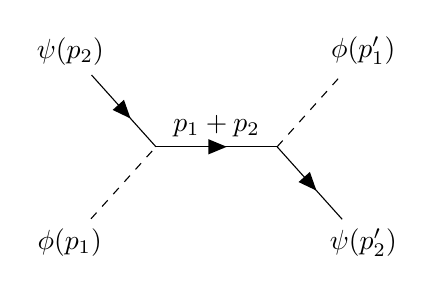
\begin{tikzpicture}
\begin{feynman}
\diagram [horizontal=a to b] {
i1 [particle=\(\phi(p_1)\)] -- [scalar] a -- [fermion, edge label=\(p_1+p_2\)] b -- [scalar] f1 [particle=\(\phi(p_1')\)],
i2 [particle=\(\psi(p_2)\)] -- [fermion] a,
b -- [fermion] f2 [particle=\(\psi(p_2')\)],
};
\end{feynman}
\end{tikzpicture}
\caption{\(s\)-channel contribution to \(\phi+\psi\to\phi+\psi\)}
\end{figure}

\begin{figure}[h!]
\centering
\begin{tikzpicture}
\begin{feynman}
\diagram [horizontal=a to b] {
i1 [particle=\(\phi(p_1)\)] -- [scalar] a,
i2 [particle=\(\psi(p_2)\)] -- [fermion] a -- [fermion, edge label=\(p_2-p_1'\)] b -- [fermion] f2 [particle=\(\psi(p_2')\)],
a -- [scalar] f1 [particle=\(\phi(p_1')\)],
};
\end{feynman}
\end{tikzpicture}
\caption{\(u\)-channel contribution to \(\phi+\psi\to\phi+\psi\)}
\end{figure}

\end{document}